\section{The Flatten-Then-Project Readout is Rank-Blind}
\label{sec:flat}

\subsection{Four flat rank-$k$ curves}

We ran the matrix bottleneck under four training conditions that
vary the task, the CODI distillation weight $\gamma$, and the
multiplicative thinker. Each run produced a single rank-$k$ ablation
curve.

\begin{table}[t]
\caption{Rank-$k$ projection ablation across four training
conditions. $\Z$ rank is the mean effective rank of the $16\times16$
matrix thought at eval time. $r_s$ is the Spearman rank correlation
between per-sample effective rank and correctness. Range across
$k\in\{1,2,4,8,16\}$ is $\leq 0.6$pp in every row. R1 (GSM8K-Aug)
is at a $6\%$ operating point below the learning threshold and is
not interpretable on its own.}
\label{tab:four-flat}
\centering
\footnotesize
\setlength{\tabcolsep}{2pt}
\begin{tabular}{llcclccc}
\toprule
Run & Task & $\gamma$ & Thinker & $\Z$ rank & k{=}1 & k{=}16 & $r_s$ \\
\midrule
R1 & GSM8K-Aug & 1.0 & on  & 5.5  & 6.00\% & 6.12\% & $-0.023$ \\
R2 & ProsQA    & 1.0 & on  & 10.2 & 78.4\% & 78.4\% & $+0.026$ \\
R3a & ProsQA   & 0.0 & on  & 12.7 & 76.8\% & 76.6\% & $-0.105$ \\
R3b & ProsQA   & 0.0 & off & 12.8 & 72.6\% & 72.4\% & $+0.095$ \\
\bottomrule
\end{tabular}
\end{table}

Varying the task (arithmetic vs.\ logical), the distillation weight
(removing the L1-at-colon loss raises effective rank from
$\sim\!10$ to $\sim\!13$ but leaves the curve shape unchanged), or
the multiplicative thinker (off drops accuracy by $\sim\!1$pp; curve
still flat) does not bend any of the four curves. A vanilla GPT-2 SFT
model with no $\Z$ at all also produces a flat curve under the same
probe (\S\ref{sec:pc-negctrl}). The three-seed decoupling result
(Fig.~\ref{fig:seed-decoupling}) below is the model-level evidence
the negative control cannot reproduce by construction.

\subsection{Why: the readout Jacobian is constant in $\Z$}

The flatten-then-project readout is
$\phi(\Z) = W_{\text{down}}\vecop(\Z)$. Its Jacobian with respect
to $\vecop(\Z)$ is the constant matrix $W_{\text{down}}$:
\[
\frac{\partial\phi}{\partial\vecop(\Z)} \;=\; W_{\text{down}}.
\]
By the chain rule, the loss gradient is
\[
\frac{\partial\mathcal{L}}{\partial\vecop(\Z)}
\;=\;
W_{\text{down}}^{\top}\,
\frac{\partial\mathcal{L}}{\partial\phi}.
\]
The pullback factor $W_{\text{down}}^{\top}$ is independent of
$\Z$. Any $\Z$-dependence of the gradient enters only through the
upstream factor $\partial\mathcal{L}/\partial\phi$, which depends
on $\Z$ only through the value $\phi(\Z)$, not through any
explicit factor of $\Z$'s SVD basis.

\begin{proposition}[Linear readout has constant Jacobian]
\label{prop:jac}
Let $\phi:\R^{d\times d}\to\R^{D}$ be linear in $\Z$. The Jacobian
$\partial\phi/\partial\vecop(\Z)$ is a constant matrix
$W\in\R^{D\times d^2}$, and the loss gradient is
$\partial\mathcal{L}/\partial\vecop(\Z) = W^{\top}\,\partial\mathcal{L}/\partial\phi$.
The pullback factor $W^{\top}$ is independent of $\Z$. Any
rank-dependence of $\partial\mathcal{L}/\partial\Z$ enters only
through the upstream factor $\partial\mathcal{L}/\partial\phi$,
which sees $\Z$ only through $\phi(\Z)$. The chain rule therefore
introduces no term that couples directly to the SVD basis of
$\Z$; the loss has no built-in rank reward. Implicit bias from the
optimizer (Adam $+$ weight decay) and upstream regularization may
still shape rank through channels outside $\mathcal{L}$
(\S\ref{sec:related}).
\end{proposition}

\begin{proof}[Proof sketch]
Differentiating $\phi(\Z) = W\,\vecop(\Z)$ gives
$\partial\phi/\partial\vecop(\Z) = W$, a constant matrix. The
chain rule then yields
$\partial\mathcal{L}/\partial\vecop(\Z) = W^{\top}\,\partial\mathcal{L}/\partial\phi$;
the prefactor $W^{\top}$ does not depend on $\Z$. \qedhere
\end{proof}

\paragraph{Remark.} The proposition is a statement about the
chain-rule pullback, not about the full $\Z$-dependence of the
gradient. Different $\Z$'s produce different
$\partial\mathcal{L}/\partial\phi$ and therefore different
gradients. What is ruled out is an SVD-basis-dependent term in
the chain rule itself. Whether the absence of an explicit rank
preference yields rank-blind behavior in practice is an empirical
question; \S\ref{sec:pc} tests it by replacing $\phi$ with
nonlinear functions, and the flat curves persist, suggesting
at least part of the explanation lies elsewhere.

The four training conditions in Table~\ref{tab:four-flat} are
consistent with the proposition's prediction for linear $\phi$.
\S\ref{sec:pc} tests what happens when the linearity premise is
violated.

\subsection{Accuracy is decoupled from rank across seeds}

Proposition~\ref{prop:jac} predicts that the loss landscape should
be flat along rank-changing directions of $\Z$: a model ending
training at rank $12$ and a model ending at rank $4$ can achieve the
same accuracy. We test this with three training seeds of the same
flatten-readout configuration (gpt2-small, ProsQA, $\gamma=0$, 25
epochs, batch 16).

\begin{figure}[t]
\centering

\includegraphics[width=\linewidth]{figures/fig2_seed_decoupling.pdf}
\caption{Three-seed replication of the flatten readout. Best ProsQA
accuracy is tight at $81.51\pm 1.2$pp, but the final effective rank
of $\Z$ varies $3\times$: seed 42 converges at rank $\sim\!4$;
seeds 1337 and 7 converge near rank $12$. The loss does not push
$\Z$ toward any particular rank.}
\label{fig:seed-decoupling}
\end{figure}

\subsection{Linear probe on $\Z$}

If rank is vestigial, what \emph{does} $\Z$ carry? A 5-fold
cross-validated multi-class logistic regression predicts the ProsQA
target class from a flattened $\Z$ on $500$ held-out test problems.
Controls: the same prompt's hidden state from a pretrained GPT-2
with no ProsQA fine-tuning, and the same model at random
initialization.

\begin{figure}[t]
\centering
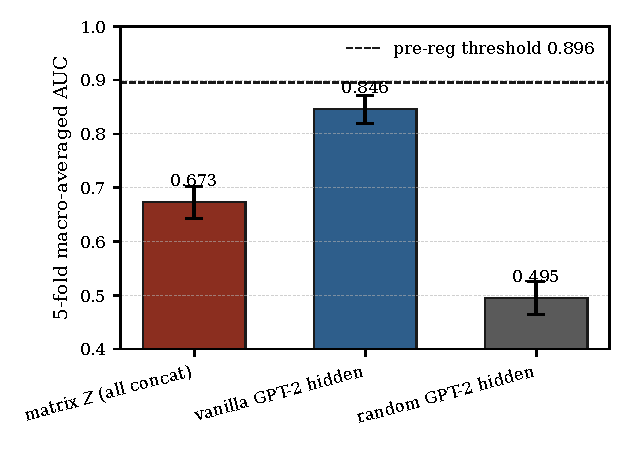
\includegraphics[width=\linewidth]{figures/fig5_linear_probe.pdf}
\caption{Linear probe AUC for ProsQA target class prediction.
Pre-registered threshold for a positive result was
$\max(\text{vanilla},\text{random})+0.05=0.896$. The matrix $\Z$
concat AUC of $0.673$ does not exceed it. Vanilla GPT-2, never
trained on ProsQA, predicts the target class better than the
trained matrix-CODI bottleneck.}
\label{fig:probe}
\end{figure}

Vanilla pretrained GPT-2 reaches AUC $0.846$ at 768 features. The
matrix-CODI bottleneck's concatenated matrix thought (6 latent
positions $\times$ 256 features $= 1536$ features) reaches AUC
$0.673$: more features than the vanilla hidden state, lower
predictive signal for the ProsQA target. A dimension-matched
comparison (probe on the post-bottleneck reconstructed 768-dim
hidden state $W_{\text{down}}\vecop(\Z)$ that the downstream
transformer consumes) is pending. A binary target-vs-distractor
probe on the same $\Z$ tensors is at chance (AUC $0.50$--$0.56$)
across all conditions.
